\begin{figure}
\centering
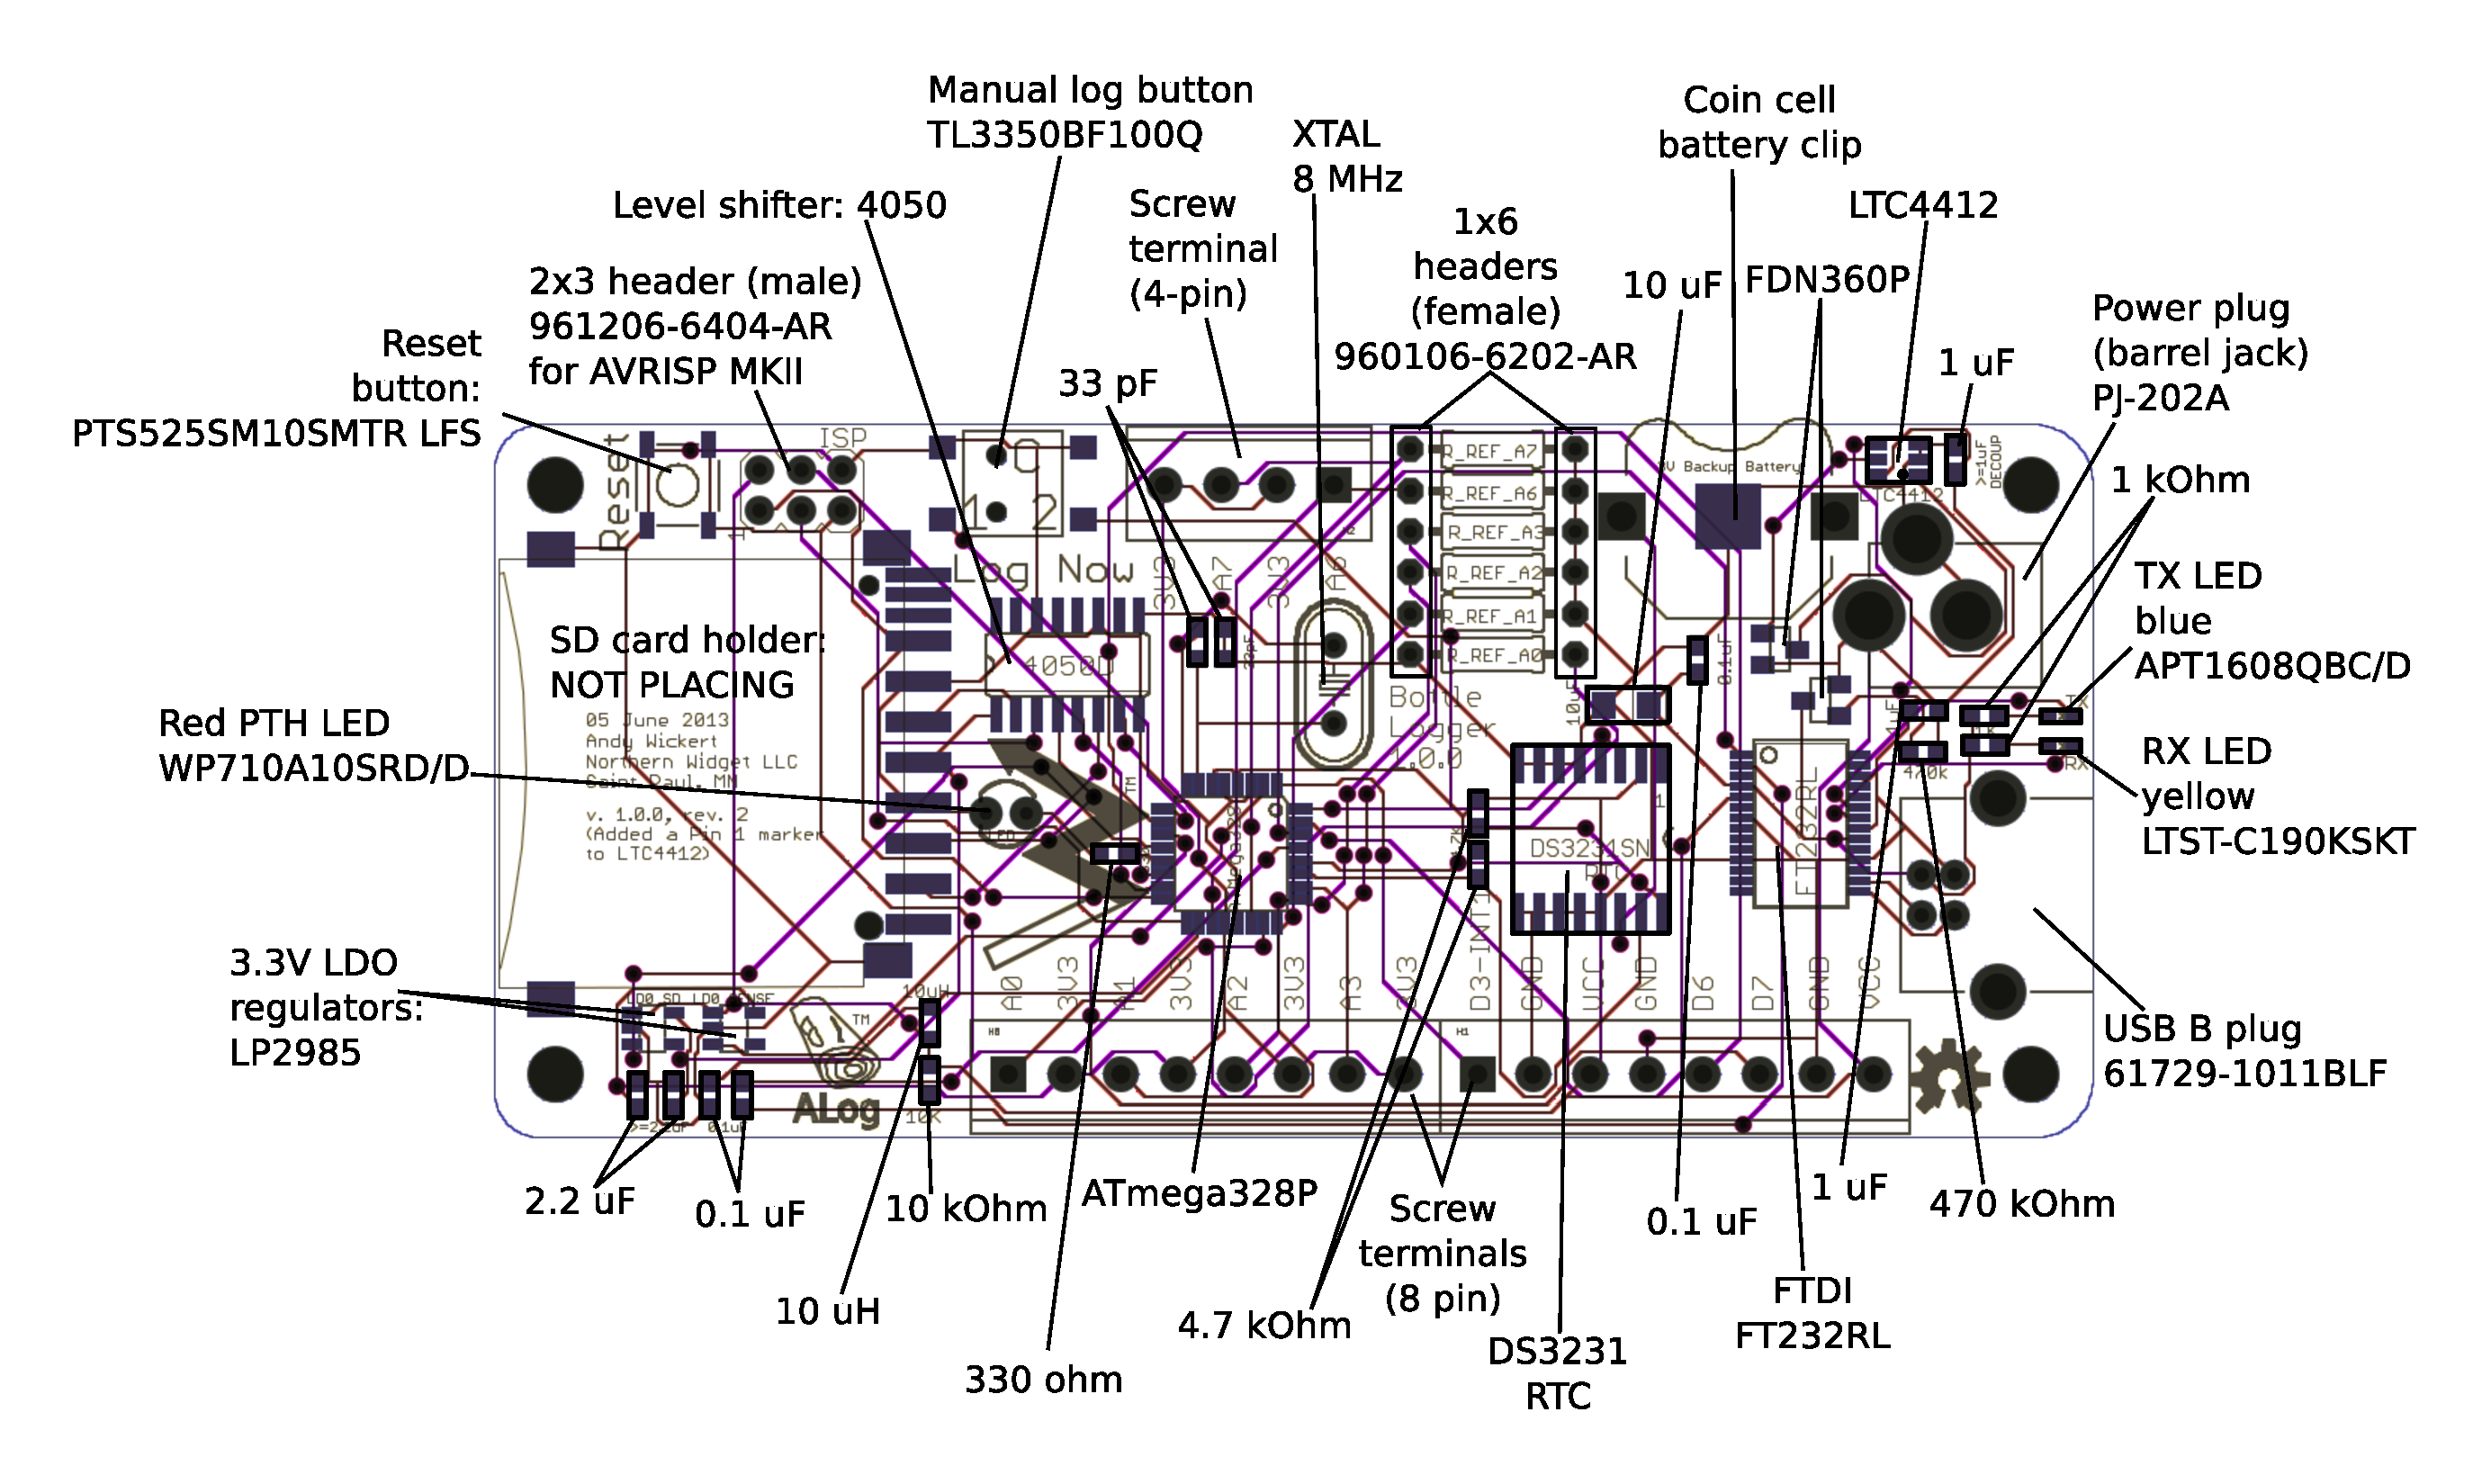
\includegraphics[height=10cm]{graphics/ALog_drawing}
\caption{Arduino-based low-power field environmental data logging platform: hardware schematics and circuit board layouts\label{fig:BottleLog}\cite{ALog-BottleLogger}}
\end{figure}

\section{Background}
Data sampling is well know method to help scientist to understand nature's behavior. Back in days, scientist had to sample data in real time on the field by writing measurements down to log book. Later on with automatic measurement equipment they where able to leave it behind in the field, then come back later and collect the data from them to process. Later on with impact of wireless communication technology the automatic measurement equipment the scientist were able to access data in real time to process.\\
Similar equipment that is available to day that fulfills the requirements of being light-weight, inexpensive and has long-range transmit capabilities is not available. The equipment that is capable of long range communications through GSM network can be seen in figures \ref{fig:a} and \ref{fig:b} and they cost about \$3000. Then there is cheaper equipment that costs around \$500 as in figures\ref{fig:c} and  \ref{fig:d} but the downfall with them is that they have limited wireless range up to 300 m.

\begin{figure}[H]
  \centering
  \subfloat[\$3500 \label{fig:a}\cite{WeatherShop2014}]
  {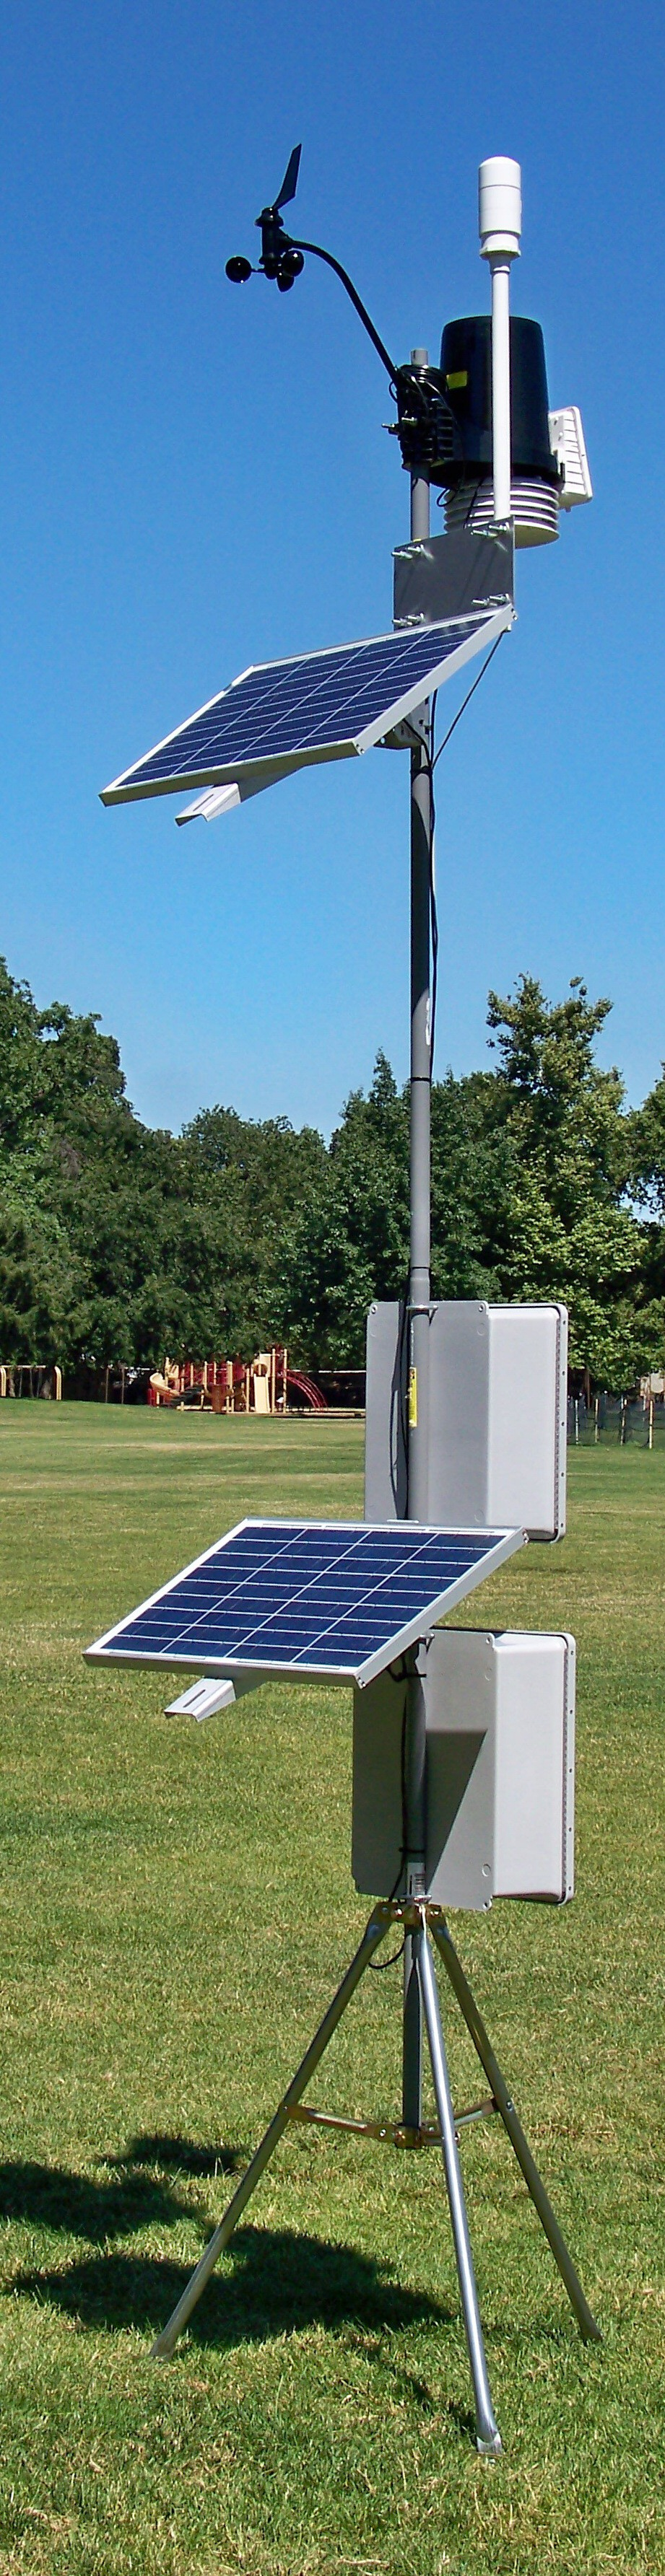
\includegraphics[height=6.5cm]{graphics/cellular_weather_station}}\quad
  \subfloat[\$2800 \label{fig:b}\cite{TexasWeatherInstruments2014}]
  {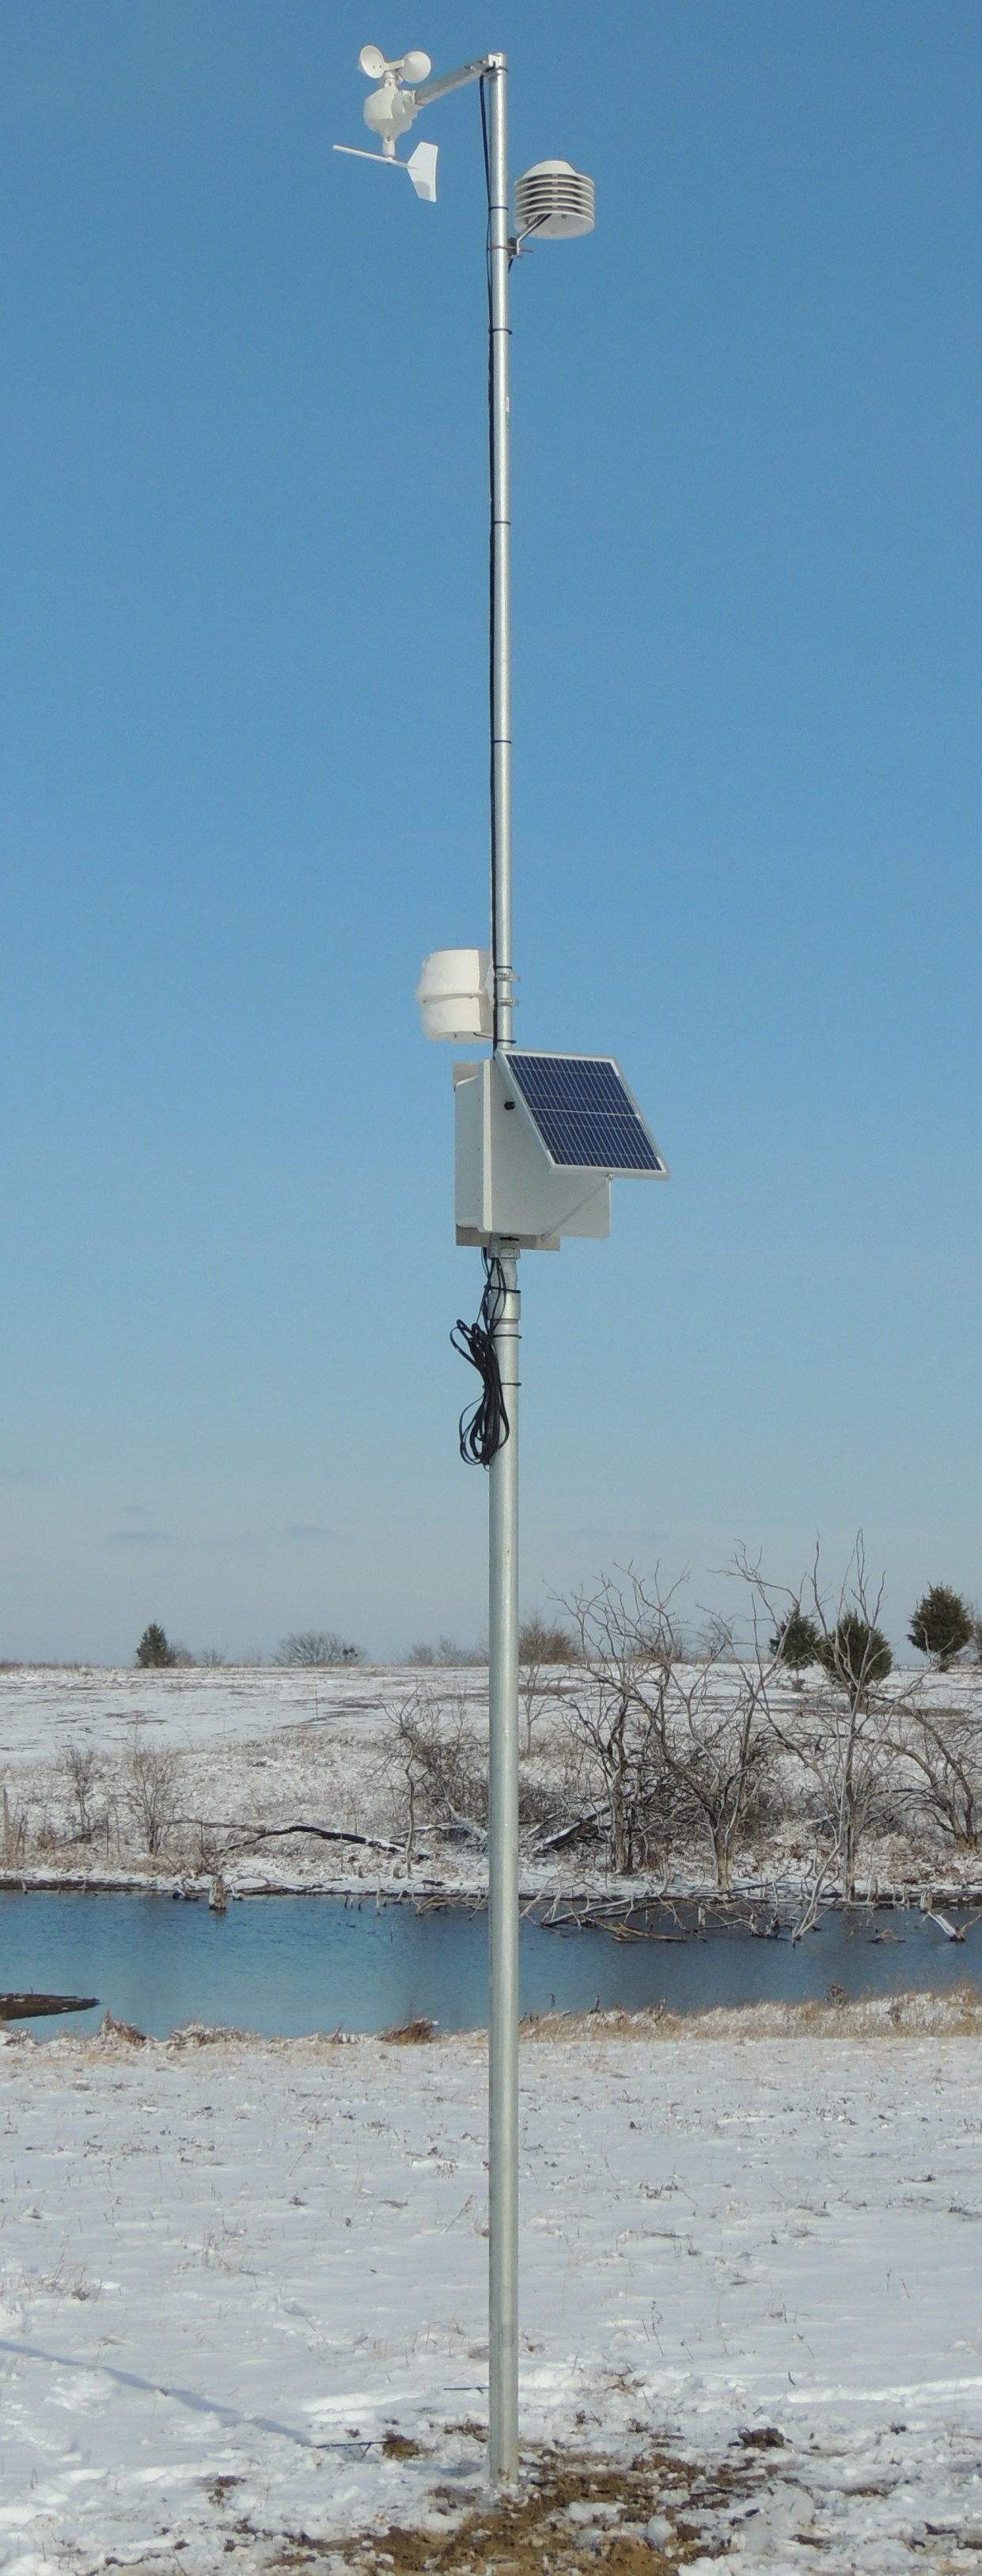
\includegraphics[height=6.5cm]{graphics/RWS-Snow}}\quad
  \subfloat[\$658 \label{fig:c}\cite{Scientific2014}]
  {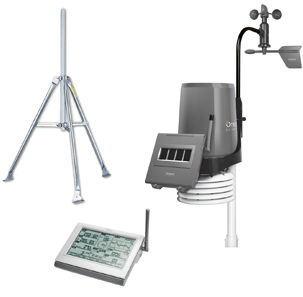
\includegraphics[height=4cm]{graphics/Oregon_Scientific_Pro_weather_system}}\quad
  \subfloat[\$595 \label{fig:d}\cite{Davis2014}]
  {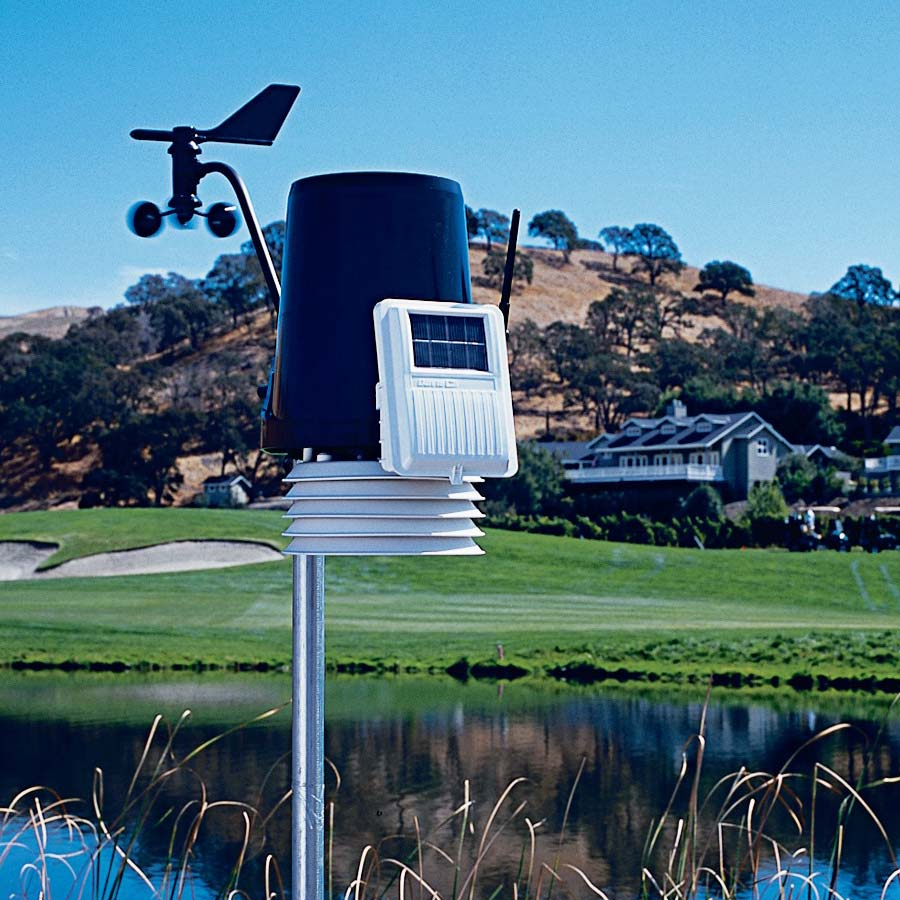
\includegraphics[height=4cm]{graphics/Davis_Vantage_Pro_2}}  
  \caption{Various price of portable weather stations}
  \label{fig:1}
\end{figure}

With that in mind the concept with this project is to make long-range communication data logger that is affordable. That can have good impact on the scientific communities were budgets are often limited. It can also result in more dens coverage in data logging. 